\documentclass[11pt]{article}
\usepackage{graphicx}
\usepackage{hyperref}
\usepackage{natbib}
\usepackage{setspace}

\setlength{\textwidth}{6.5in}
\setlength{\headheight}{0in}
\setlength{\textheight}{8.0in}
\setlength{\hoffset}{0in}
\setlength{\voffset}{0in}
\setlength{\oddsidemargin}{0in}
\setlength{\evensidemargin}{0in}
\doublespacing

\title{Computational Physics HW2}
  
\author{Siyuan Chen}


\begin{document}

\maketitle

\section*{}
P1:
Numpy.float32 represents a real number with 32-digit of binary numbers. It approximates the number to be the form of $\pm(1+\sum\limits^{22}_{i=0}m_i2^{-(i-23)})2^{e-127}$ then represents it with the nearest mantissa $m_i$ and exponent $e$ from the format. In the 32-digit of binary numbers, the first digit on the left represents the positive or negative sign; the following 8 digit is the binary form of the exponent $e$; the last 23 digit are the mantissa $m$s. In this method, 100.98763 is represented by 01000010110010011111100110101011. The round-off error of such representation is about $2.7514648479609605\times10^{-6}$.

\section*{}
P2:
From the equation given in Exercise 2.9, we can cancel the physical constants on both sides and get $M=\sum\limits^L_{i,j,k=-L}(-1)^{i+j+k}\frac{1}{\sqrt{i^2+j^2+k^2}}$, not i=j=k=0. In the first method, we write a for loop to add the potentials from atoms at different positions on the grid. In the second method, we write coordinates of the grid and calculate potentials as an array-like object. Notice here we have to use floating point data type to record coordinates such that certain calculations could be allowed. For L = 100, the time to execute for loop is about 40s whereas for grid method, it's only 0.25s. Both methods agree the Madelung constant for sodium in sodium chloride to be -1.7418.

\section*{}
P3:

\begin{figure}
    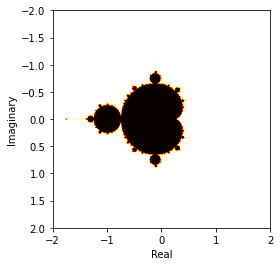
\includegraphics{Mandelbrot.png}
    \caption{\textbf{Mandelbrot} 
    }
    \label{fig}
\end{figure}

\end{document}

 
 
